\documentclass[aspectratio=169,11pt,t]{beamer}
% ============================================================
%  ksa-cs-v2: ksa-cs-lecture-template.tex 스타일 + 한글, v2 덱(16:9)용.
%    - 짙은 네이비 헤드라인 (섹션 이름 + 프레임마다 점)
%    - 꽉 찬 파란 제목 막대, 둥근 그림자 블록
%    - 한글: Noto Sans CJK KR (fontspec)
%  사용:
%    \documentclass[aspectratio=169,11pt,t]{beamer}
%    \input{<..>/theme/ksa-cs-v2.tex}
%  ksa-theme.tex 의 매크로(\kb \kq, ksablue/ksared 등)도 같은 이름으로 둔다
%  -> v2 덱 본문을 거의 그대로 옮길 수 있다.
% ============================================================

\usepackage{fontspec}
\usepackage{amsmath,amssymb}
\usepackage{tikz}
\usepackage{listings}
\usepackage{graphicx}
\usepackage{booktabs}
\usepackage{varwidth}
% enumitem 은 넣지 않는다 (beamer 글머리표가 사라진다)

\defaultfontfeatures{Ligatures=TeX}
\setmainfont{Noto Sans CJK KR}
\setsansfont{Noto Sans CJK KR}
\setmonofont{Noto Sans Mono CJK KR}[Scale=0.92]
\usefonttheme{professionalfonts}

% ---------- 기본 틀 ----------
\usetheme{default}
\useinnertheme[shadow=true]{rounded}
\setbeamertemplate{navigation symbols}{}
\setbeamersize{text margin left=1em,text margin right=1em}

% ---------- 색 (템플릿 원본 값) ----------
\definecolor{navydark}{HTML}{191959}
\definecolor{navydim}{HTML}{8888B0}
\definecolor{navytitle}{HTML}{262686}
\definecolor{navyblue}{HTML}{3333B2}
\definecolor{blockbodybg}{HTML}{E9E9F3}
\definecolor{examplegreen}{HTML}{006000}
\definecolor{examplebg}{HTML}{E5EFE5}
\definecolor{alertred}{HTML}{BF0000}
\definecolor{alertbg}{HTML}{F9E5E5}
% ksa-theme.tex 와 같은 이름 (본문 호환)
\colorlet{ksablue}{navytitle}
\colorlet{ksabluedk}{navydark}
\definecolor{ksagold}{HTML}{D6CBB1}
\definecolor{ksagolddk}{HTML}{A9976B}
\colorlet{ksared}{alertred}
\definecolor{ksagray}{HTML}{5B5B5B}

\setbeamercolor{structure}{fg=navyblue}
\setbeamercolor{alerted text}{fg=alertred}
\setbeamercolor{frametitle}{bg=navytitle,fg=white}
\setbeamercolor{title}{fg=white,bg=navytitle}
\setbeamercolor{block title}{bg=navytitle,fg=white}
\setbeamercolor{block body}{bg=blockbodybg,fg=black}
\setbeamercolor{block title example}{bg=examplegreen,fg=white}
\setbeamercolor{block body example}{bg=examplebg,fg=black}
\setbeamercolor{block title alerted}{bg=alertred,fg=white}
\setbeamercolor{block body alerted}{bg=alertbg,fg=black}
\setbeamercolor{item}{fg=navyblue}
\setbeamertemplate{itemize item}[circle]
\setbeamertemplate{itemize subitem}[triangle]

% ---------- 헤드라인: miniframes (섹션 이름 + 점) ----------
\useoutertheme[subsection=false]{miniframes}
\setbeamerfont{section in head/foot}{size=\tiny}
\setbeamercolor{section in head/foot}{bg=navydark,fg=white}
\setbeamercolor{mini frame}{fg=white}
\setbeamertemplate{mini frames}[circle]

% ---------- 제목 막대: 폭 꽉 채움, 두 줄까지 ----------
\setbeamerfont{frametitle}{size=\normalsize,series=\bfseries}
\setbeamertemplate{frametitle}{%
  \nointerlineskip
  \begin{beamercolorbox}[wd=\paperwidth,ht=2.7ex,dp=1.1ex,leftskip=.3cm,rightskip=.3cm]{frametitle}%
    \usebeamerfont{frametitle}\insertframetitle
  \end{beamercolorbox}}

% ---------- 쪽 번호: 오른쪽 아래 ----------
\setbeamertemplate{footline}{%
  \hfill
  {\color{navydim}\scriptsize\insertframenumber\,/\,\inserttotalframenumber}%
  \hspace{3mm}\vspace{2mm}%
}

% ---------- 표지: 템플릿처럼 헤드라인은 그대로, 가운데 둥근 그림자 상자에 제목 한 줄 ----------
% 덱에서:  {\setbeamertemplate{footline}{}\begin{frame}[c,noframenumbering]\titlepage\end{frame}}
\setbeamercolor{title}{fg=white,bg=navyblue}
\makeatletter
\setbeamertemplate{title page}{%
  \vfill
  \centering
  \begin{minipage}{0.84\paperwidth}
  \begin{beamercolorbox}[wd=\linewidth,sep=7pt,center,rounded=true,shadow=true]{title}
    {\usebeamerfont{title}\inserttitle\par}%
    \ifx\insertsubtitle\@empty\else\vskip0.4em{\usebeamerfont{subtitle}\insertsubtitle\par}\fi
  \end{beamercolorbox}
  \end{minipage}\par\vskip1.6em
  {\usebeamerfont{author}\color{navytitle}\insertauthor\par}\vskip0.3em
  {\usebeamerfont{institute}\color{ksagray}\insertinstitute\par}
  \vfill
}
\makeatother
\setbeamerfont{title}{series=\bfseries,size=\Large}
\setbeamerfont{subtitle}{size=\normalsize}
\setbeamerfont{author}{size=\normalsize}
\setbeamerfont{institute}{size=\small}

% ksa-theme 호환: 덱이 \renewcommand{\ksacredit}{..} 를 해도 되게 (꼬리말에는 안 쓴다)
\newcommand{\ksacredit}{}

% ---------- 강조 ----------
\newcommand{\hl}[1]{\textcolor{alertred}{#1}}
\newcommand{\hlb}[1]{\textcolor{navyblue}{#1}}
\newcommand{\kb}[1]{\textbf{\color{ksablue}#1}}
\newcommand{\kq}[1]{\textbf{\color{ksared}#1}}

% ---------- 파이썬 코드 (템플릿과 같은 색) ----------
\definecolor{codekw}{HTML}{0033B3}
\definecolor{codebuiltin}{HTML}{BF0000}
\definecolor{codestr}{HTML}{067D17}
\definecolor{codecomment}{HTML}{8C8C8C}
\definecolor{codenum}{HTML}{1750EB}
\lstdefinestyle{py}{
  language=Python, basicstyle=\ttfamily\scriptsize,
  keywordstyle=\color{codekw}\bfseries, stringstyle=\color{codestr},
  commentstyle=\color{codecomment}\itshape, numberstyle=\color{codenum},
  emph={print,len,range,sum,input,int,str,float,list,dict,append,remove,sorted,abs,min,max},
  emphstyle=\color{codebuiltin}, showstringspaces=false, keepspaces=true,
  columns=fixed, basewidth=0.52em, aboveskip=1mm, belowskip=1mm, xleftmargin=2mm,
  breaklines=true
}
\lstset{style=py}

% 원본 덱 (ksa-theme): slides/v2/ml1/week02/sgd/ -- 그림은 거기 figs/ 를 그대로 쓴다
\setbeamerfont{author}{size=\normalsize}
\setbeamerfont{institute}{size=\small}
\graphicspath{{figs/}{../../../v2/ml1/week02/sgd/figs/}{../../../assets/}}
% 쪽 참조: \markpage{이름} 을 프레임 안에 두고, 다른 곳에서 \pref{이름} 으로 (p.N) 을 부른다 (하단 번호와 같은 번호, 클릭하면 이동)
\makeatletter
\newcommand{\markpage}[1]{\protected@write\@auxout{}{\string\newlabel{#1}{{\the\c@framenumber}{}}}\hypertarget{#1}{}}
\newcommand{\pref}[1]{\hyperlink{#1}{\textcolor{ksagolddk}{(p.\ref{#1})}}}
\makeatother

\renewcommand{\ksacredit}{Machine Learning and Deep Learning \,\textperiodcentered\, 확률적 경사하강법}
\title{확률적 경사하강법 (SGD)}
\subtitle{일부만 보고 자주 걷는 경사하강법}
\author{Machine Learning and Deep Learning}
\institute{한국과학영재학교 (KSA)}
\date{}
\begin{document}
{\setbeamertemplate{footline}{}\begin{frame}[c,noframenumbering]\titlepage\end{frame}}

\section{질문}
% --- 오늘의 질문
\begin{frame}{오늘의 질문}
\vfill
\centering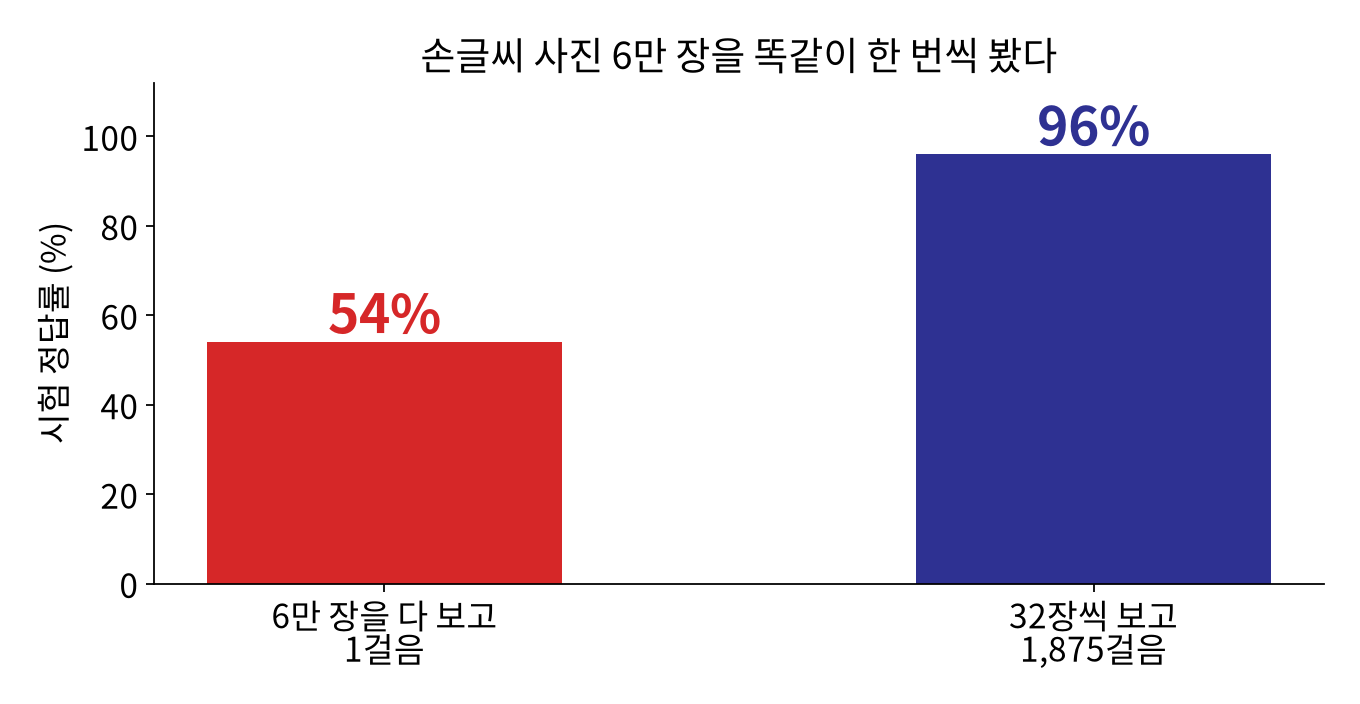
\includegraphics[height=0.36\textheight]{sgd_hook.png}\par\vskip0.2em
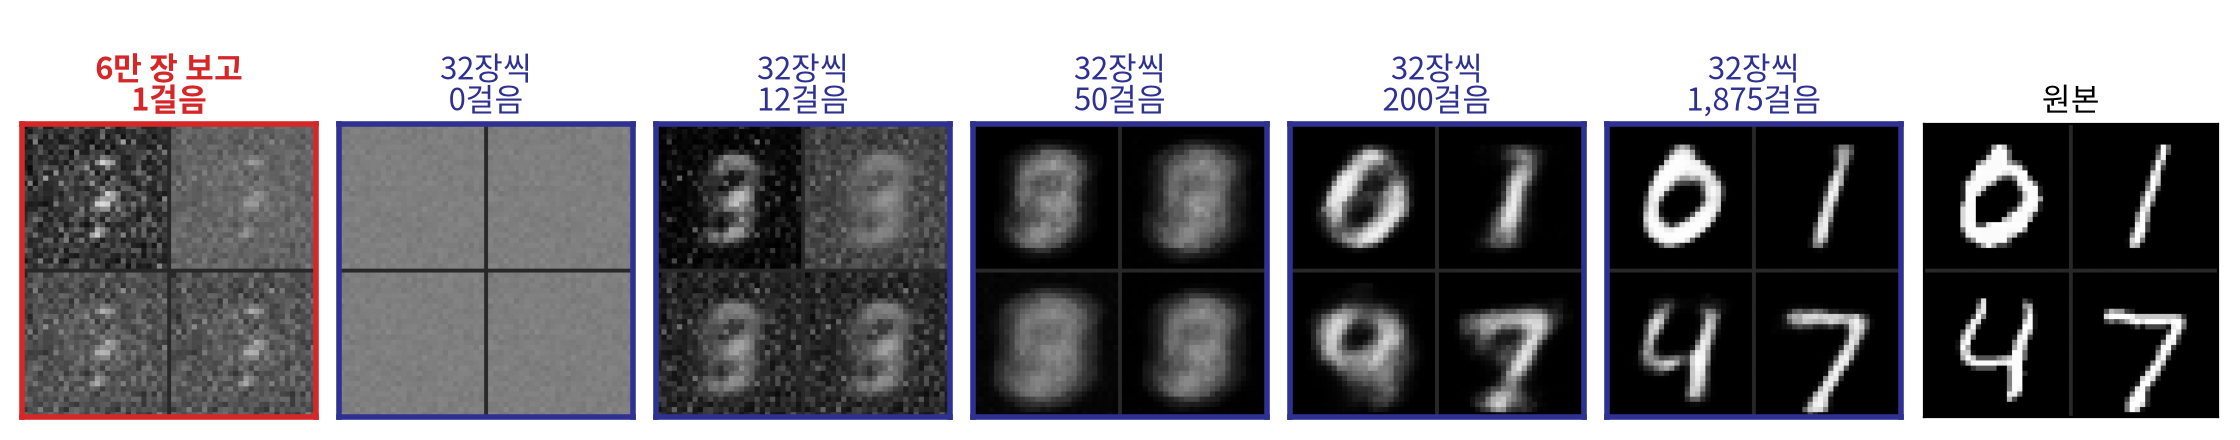
\includegraphics[width=0.86\linewidth]{sgd_ae_steps.png}\par\vskip0.2em
{\small 같은 손글씨 사진 6만 장(MNIST)을 한 번씩. 위: 숫자 맞히기 \,·\, 아래: 숫자 다시 그리기(오토인코더)}\\[0.2em]
\kq{SGD: 6만 장 $=$ 32장 $\times$ 1,875걸음}
\vfill
\note{손글씨 숫자 사진 6만 장으로 같은 신경망을 두 번 학습시켰습니다. 두 번 모두 사진을 정확히 한 번씩 봤습니다. 그런데 한쪽은 시험 정답률 54퍼센트, 다른 쪽은 96퍼센트입니다. 차이는 기울기를 구하는 방법 하나뿐입니다. 왼쪽은 1주차에 배운 경사하강법 그대로, 6만 장을 다 보고 한 걸음 갔습니다. 오른쪽은 32장씩 보고 바로바로 걸어서 1,875걸음을 갔습니다. 6만 장은 32장씩 1,875번 나눈 수입니다. 아래는 숫자를 보고 똑같이 다시 그리는 신경망, 오토인코더입니다. 이번에도 6만 장을 한 번씩만 봤습니다. 6만 장을 다 보고 한 걸음 간 빨간 칸은 아직 지지직거리는 잡음입니다. 32장씩 걸으면 처음엔 회색, 12걸음쯤엔 뿌연 덩어리, 200걸음이면 0, 1, 4, 7 이 보이고, 1,875걸음 끝에는 원본과 거의 같아집니다. 오늘은 오른쪽 방법, 확률적 경사하강법을 배웁니다.}
\end{frame}

\section{복습}
% --- 복습: 경사하강법
\begin{frame}{복습: 경사하강법}
\vfill
\centering{\LARGE\[ w \;\leftarrow\; w - \alpha\,\frac{\partial J}{\partial w}\]}\vskip0.6em
$\alpha$: 학습률 (한 걸음의 크기) \qquad $\dfrac{\partial J}{\partial w}$: 비용이 늘어나는 방향\\[1.0em]
\kq{한 걸음마다 $\dfrac{\partial J}{\partial w}$ 를 새로 구한다}
\vfill
\note{1주차에 배운 경사하강법입니다. 비용 J가 늘어나는 방향, 즉 기울기를 구해서 그 반대 방향으로 학습률 알파만큼 걷습니다. 중요한 건 한 걸음마다 기울기를 새로 구해야 한다는 점입니다. 걸음을 옮기면 서 있는 위치가 바뀌고, 기울기도 바뀌기 때문입니다. 그러면 기울기 한 번을 구하는 데 얼마나 걸릴까요?}
\end{frame}

% --- 비용은 평균, 기울기도 평균
\begin{frame}{비용은 평균, 기울기도 평균}
\markpage{avggrad}
\vfill
\centering{\LARGE\[ J(w) = \frac{1}{m}\sum_{i=1}^{m} \ell_i(w) \qquad\Rightarrow\qquad \frac{\partial J}{\partial w} = \frac{1}{m}\sum_{i=1}^{m} \frac{\partial \ell_i}{\partial w}\]}\vskip0.6em
$\ell_i$: 데이터 $i$ 하나의 손실 \qquad $m$: 데이터 수\\[0.8em]
\kb{전체 기울기 = 데이터 하나하나의 기울기의 평균}
\vfill
\note{비용 J는 데이터 하나하나의 손실을 평균한 것입니다. 미분은 더하기와 순서를 바꿔도 되니까, 기울기도 데이터 하나하나의 기울기를 평균한 것이 됩니다. 그러니까 기울기를 한 번 구하려면 데이터 m개의 기울기를 전부 구해서 평균해야 합니다. 이 식이 오늘 수업의 출발점입니다.}
\end{frame}

% --- 가장 단순한 모델로 세어 보기
\begin{frame}{가장 단순한 모델로 세어 보기}
\vfill
\centering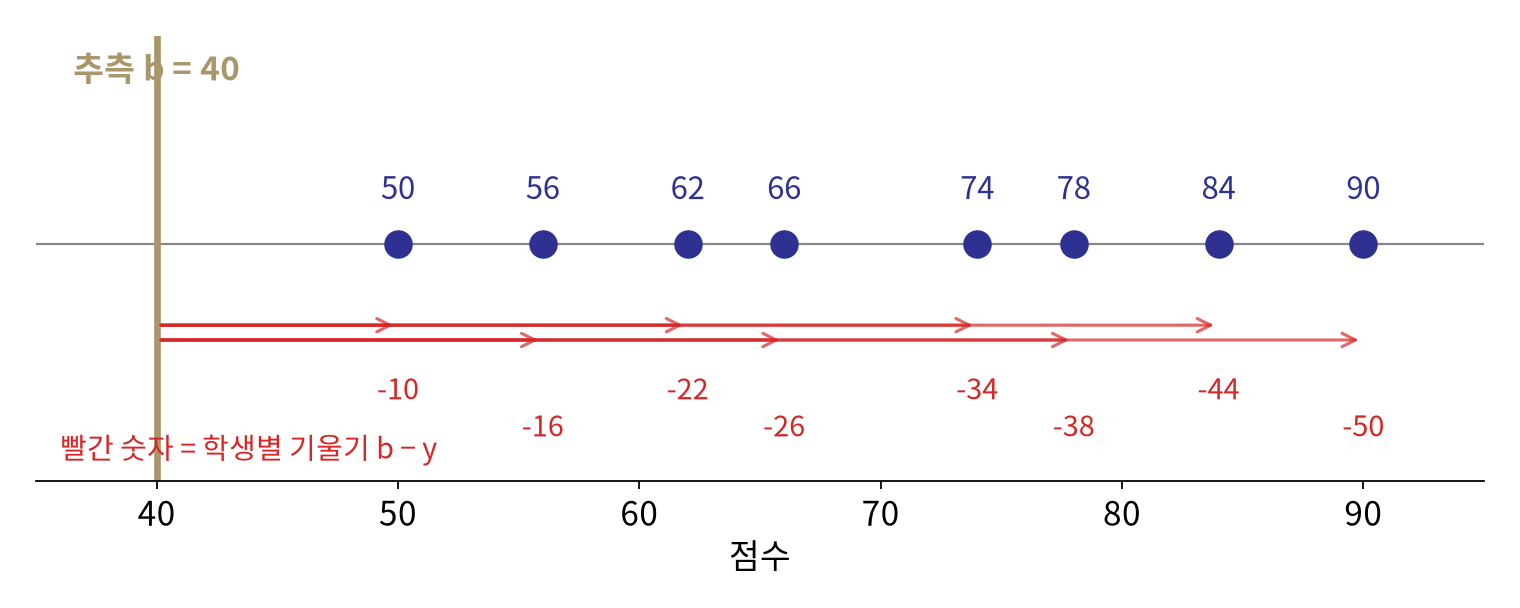
\includegraphics[width=0.84\linewidth]{sgd_scores.png}\par\vskip0.2em
{\normalsize 모델 $\hat y = b$ (숫자 하나로 8명의 점수를 맞힌다) \quad 손실 $\ell_i = \tfrac12(b-y_i)^2$ \quad 기울기 $\dfrac{\partial \ell_i}{\partial b} = b - y_i$}
\vfill
\note{손으로 셀 수 있게 가장 단순한 모델을 씁시다. 입력 없이 숫자 하나 b로 8명의 점수를 맞히는 모델입니다. 선형회귀에서 기울기 w를 빼고 절편 b만 남긴 것이라고 보면 됩니다. 학생 i의 손실은 2분의 1 곱하기 b 빼기 y_i의 제곱이고, b로 미분하면 b 빼기 y_i입니다. 지금 추측이 40이면, 50점 학생의 기울기는 마이너스 10, 90점 학생은 마이너스 50입니다. 모두 음수이니 모두 b를 올리라고 말하고 있습니다.}
\end{frame}

% --- 전체 기울기로 한 걸음
\begin{frame}{전체 기울기로 한 걸음}
\vfill
\centering
\renewcommand{\arraystretch}{1.3}
{\normalsize\begin{tabular}{l|cccccccc}
점수 $y_i$ & 50 & 56 & 62 & 66 & 74 & 78 & 84 & 90\\\hline
기울기 $b-y_i$ & $-10$ & $-16$ & $-22$ & $-26$ & $-34$ & $-38$ & $-44$ & $-50$
\end{tabular}}\vskip1.0em
{\Large $\dfrac{\partial J}{\partial b} = \dfrac{-10-16-22-26-34-38-44-50}{8} = \kq{-30}$}\vskip0.8em
{\Large $b \;\leftarrow\; 40 - {\color{ksablue}0.5}\times(-30) = \kq{55}$}\vskip0.6em
{\small 학습률 $\alpha = {\color{ksablue}0.5}$ \quad 최적값은 평균 점수 70}
\vfill
\note{8명의 기울기를 모두 구해 평균하면 마이너스 30입니다. 학습률을 0.5로 두면 b는 40에서 0.5 곱하기 30, 15만큼 올라가 55가 됩니다. 참고로 이 모델의 최적값은 평균 점수 70입니다. 8명의 기울기를 다 구해야 한 걸음을 갈 수 있었습니다. 8명이면 금방이지만, 데이터가 많으면 어떨까요?}
\end{frame}

\section{미니배치}
% --- 문제: 데이터가 많으면?
\begin{frame}{문제: 데이터가 많으면?}
\vfill
\centering
\renewcommand{\arraystretch}{1.5}
{\Large\begin{tabular}{lr}
손글씨 숫자 MNIST & 60,000장\\
사진 분류 ImageNet & 1,281,167장
\end{tabular}}\vskip1.0em
\kq{한 걸음 = 사진 전부의 기울기를 구한 뒤에야 한 번}\\[0.6em]
{\small 학습은 보통 수천~수만 걸음이 필요하다}
\vfill
\note{손글씨 숫자 데이터 MNIST는 학습용 사진이 6만 장, 2012년 AlexNet이 학습한 ImageNet은 128만 장입니다. 경사하강법으로는 한 걸음을 가기 위해 128만 장 전부의 기울기를 구해야 합니다. 학습에는 보통 수천, 수만 걸음이 필요하니, 걸음마다 데이터 전체를 보는 건 너무 느립니다.}
\end{frame}

% --- 아이디어: 몇 명만 뽑아서 어림한다
\begin{frame}{아이디어: 몇 명만 뽑아서 어림한다}
\vfill
\centering
무작위로 2명을 뽑았다: \kb{50점, 74점}\\[1.0em]
{\Large $g_{\mathcal B} = \dfrac{(40-50)+(40-74)}{2} = \dfrac{-10-34}{2} = \kq{-22}$}\vskip1.0em
\renewcommand{\arraystretch}{1.3}
\begin{tabular}{lcc}
 & 기울기 & 방향\\\hline
8명 전체 & $-30$ & $b$ 를 올려라\\
2명 ($\mathcal B$) & $-22$ & $b$ 를 올려라
\end{tabular}\vskip0.6em
{\small $\mathcal B$: 뽑은 데이터 묶음 (미니배치) \quad 값은 다르지만 방향은 같다}
\vfill
\note{아이디어는 여론조사와 같습니다. 전국민에게 묻는 대신 일부만 뽑아 물어보듯, 데이터 전체 대신 몇 개만 뽑아 기울기를 어림합니다. 8명 중 무작위로 50점과 74점 두 명을 뽑았다고 합시다. 두 사람의 기울기를 평균하면 마이너스 22입니다. 정답인 마이너스 30과는 다르지만, b를 올리라는 방향은 같습니다. 이렇게 뽑은 묶음을 미니배치라고 하고, 기호로 B를 씁니다.}
\end{frame}

% --- 28가지 쌍을 모두 세어 보면
\begin{frame}{28가지 쌍을 모두 세어 보면}
\vfill
\centering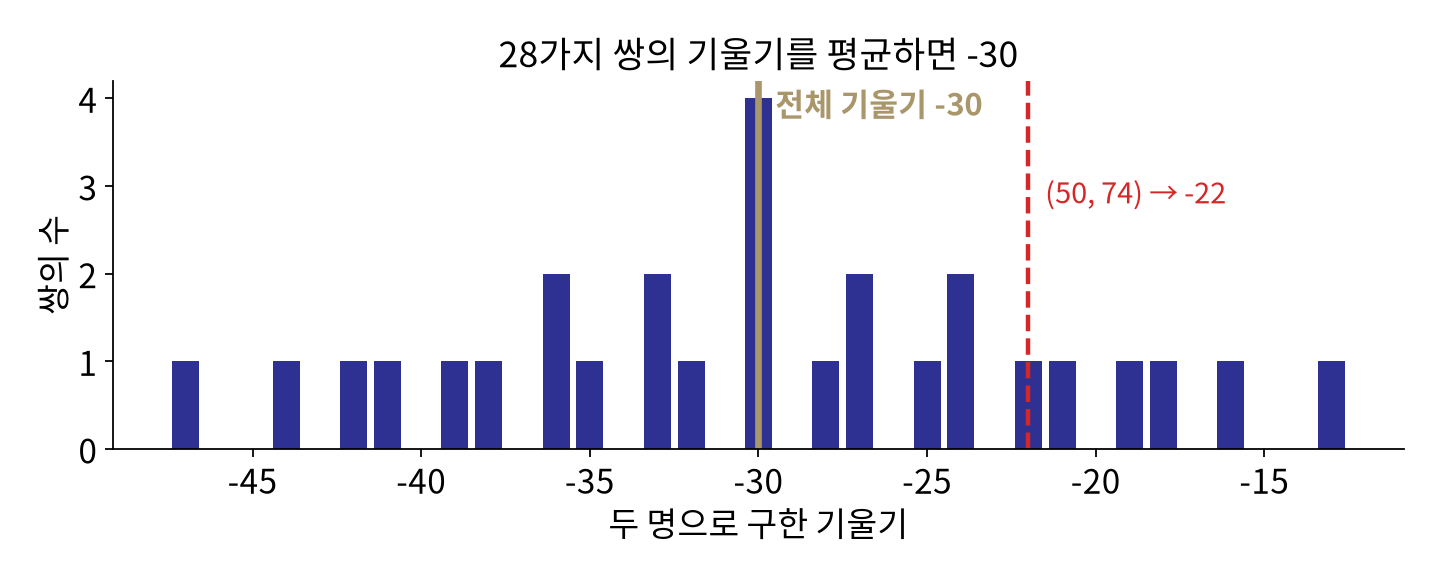
\includegraphics[width=0.74\linewidth]{sgd_pairs.png}\par\vskip0.2em
{\small 8명에서 2명을 고르는 방법 $\binom{8}{2}=28$가지 \quad 하나하나는 틀려도 \kb{평균은 정확히 $-30$}}
\vfill
\note{운이 좋았던 걸까요? 2명을 뽑는 방법 28가지를 모두 세어 봅시다. 각 쌍의 기울기는 마이너스 47부터 마이너스 13까지 흩어져 있습니다. 하지만 28개를 평균하면 정확히 마이너스 30, 전체 기울기와 같습니다. 우연이 아닙니다. 다음 쪽에서 이유를 세어 봅니다.}
\end{frame}

% --- 왜 정확히 같을까: 직접 세기
\begin{frame}{왜 정확히 같을까: 직접 세기}
\vfill
\centering
학생 한 명은 28쌍 중 \kb{7쌍}에 들어간다 \quad {\small (나머지 7명 중 짝 하나를 고른다)}\\[1.2em]
{\large $\displaystyle \frac{1}{28}\sum_{\text{28쌍}} \frac{g_a+g_b}{2} \;=\; \frac{1}{28}\cdot\frac{7}{2}\sum_{i=1}^{8} g_i \;=\; \frac{1}{8}\sum_{i=1}^{8} g_i \;=\; \frac{\partial J}{\partial b}$}\vskip1.2em
{\small $g_i = b-y_i$: 학생 $i$ 의 기울기 \quad $\dfrac{7}{2\cdot 28} = \dfrac{1}{8}$}
\vfill
\note{학생 한 명은 28쌍 가운데 몇 쌍에 들어갈까요? 나머지 7명 중 짝을 하나 고르면 되니까 7쌍입니다. 28쌍의 기울기를 모두 더하면, 학생마다 자기 기울기가 7번씩, 그리고 2로 나뉘어 들어갑니다. 그래서 합은 2분의 7 곱하기 8명 기울기의 합입니다. 이걸 28로 나누면 8분의 1 곱하기 8명 기울기의 합, 즉 전체 기울기입니다. 모든 학생이 똑같은 횟수로 뽑히기 때문에 평균이 정확히 맞는 겁니다.}
\end{frame}

% --- 유도: 미니배치 기울기의 기댓값
\begin{frame}{유도: 미니배치 기울기의 기댓값}
\vfill
\small
\begin{align*}
g_{\mathcal B} &= \frac{1}{B}\sum_{i\in\mathcal B} g_i && \text{미니배치 기울기}\\[0.3em]
\mathbb{E}\big[g_{\mathcal B}\big] &= \frac{1}{B}\sum_{i=1}^{m} P(i\in\mathcal B)\; g_i && \text{기댓값의 선형성}\\[0.3em]
&= \frac{1}{B}\sum_{i=1}^{m} \frac{B}{m}\; g_i && \text{$m$ 개 중 $B$ 개를 무작위로}\\[0.3em]
&= \frac{1}{m}\sum_{i=1}^{m} g_i \;=\; \frac{\partial J}{\partial w} && \text{\pref{avggrad}}
\end{align*}
\vskip0.3em
\centering {\normalsize $B$: 배치 크기 \quad $P(i\in\mathcal B)=\dfrac{B}{m}$: 데이터 $i$ 가 뽑힐 확률 (앞 쪽: $\tfrac{7}{28}=\tfrac{2}{8}$)}
\vfill
\note{같은 이야기를 일반적으로 써 봅시다. 미니배치 기울기는 뽑힌 B개의 기울기 평균입니다. 기댓값을 취하면, 데이터 i의 기울기는 i가 뽑힐 확률만큼 들어갑니다. m개 중 B개를 무작위로 뽑으면 i가 뽑힐 확률은 m분의 B입니다. 앞 쪽 예에서는 28쌍 중 7쌍, 즉 8분의 2였습니다. 정리하면 m분의 1 곱하기 기울기의 합, 바로 전체 기울기입니다.}
\end{frame}

% --- 결과
\begin{frame}{결과}
\vfill
\centering{\LARGE\[ \mathbb{E}\big[\,g_{\mathcal B}\,\big] = \frac{\partial J}{\partial w}\]}\vskip0.6em
미니배치 기울기는 \kb{평균적으로 정확하다}\\[0.4em]
{\small 한 번 한 번은 틀리지만, 틀리는 쪽이 한 방향으로 치우치지 않는다}
\vfill
\note{결과를 크게 봅시다. 미니배치 기울기의 기댓값은 전체 기울기와 같습니다. 한 번 한 번은 틀리지만 한쪽으로 치우쳐 틀리지 않는다는 뜻입니다. 이런 어림을 통계에서는 치우치지 않은 추정, 불편 추정이라고 부릅니다. 그러니 미니배치 기울기로 여러 번 걸으면, 흔들리긴 해도 평균적으로는 올바른 방향으로 갑니다.}
\end{frame}

% --- 몇 명을 뽑을까?
\begin{frame}{몇 명을 뽑을까?}
\vfill
\centering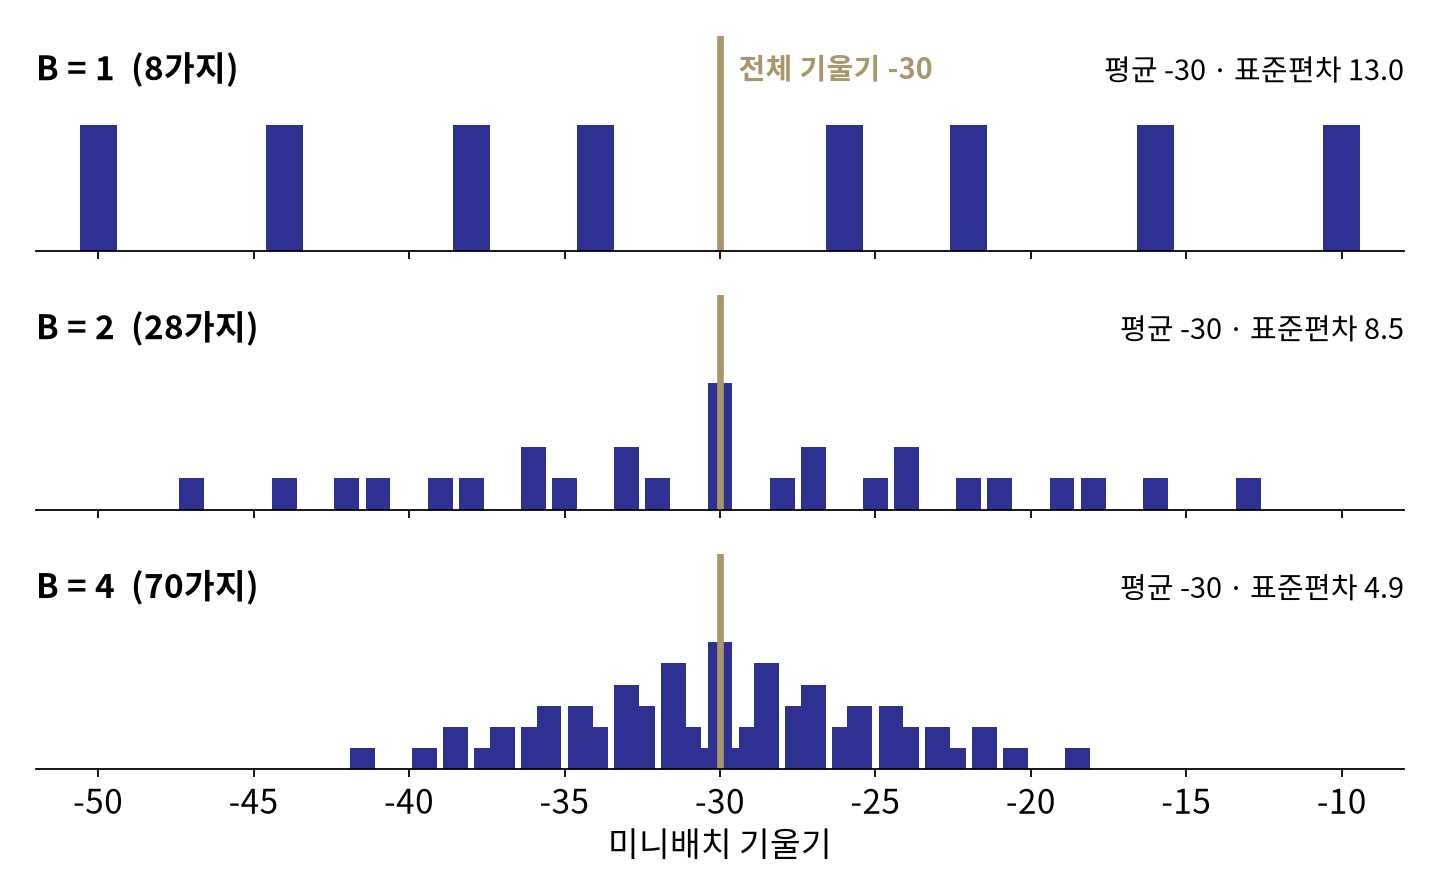
\includegraphics[width=0.62\linewidth]{sgd_spread.png}\par\vskip0.2em
{\small 평균은 늘 $-30$. 많이 뽑을수록 덜 흩어진다 \quad 표준편차 13.0 $\rightarrow$ 8.5 $\rightarrow$ 4.9}
\vfill
\note{그럼 몇 명을 뽑아야 할까요? 1명, 2명, 4명을 뽑는 모든 경우를 세어 봤습니다. 1명이면 8가지, 2명이면 28가지, 4명이면 70가지입니다. 세 경우 모두 평균은 마이너스 30으로 정확합니다. 다른 점은 흩어진 정도입니다. 표준편차가 13에서 8.5, 4.9로 줄어듭니다. 많이 뽑을수록 정확하지만, 그만큼 한 걸음에 계산이 많아집니다. 이것이 배치 크기를 고를 때의 저울질입니다.}
\end{frame}

\section{SGD}
% --- 확률적 경사하강법 (SGD)
\begin{frame}{확률적 경사하강법 (SGD)}
\markpage{algo}
\vfill
\centering
\begin{tabular}{l}
\kb{에폭마다} 데이터 $m$ 개를 섞는다\\[0.3em]
\quad 앞에서부터 $B$ 개씩 자른 미니배치 $\mathcal B$ 마다\\[0.3em]
\qquad {\Large $w \;\leftarrow\; w - \alpha\, g_{\mathcal B}$}
\end{tabular}\vskip1.0em
\renewcommand{\arraystretch}{1.3}
{\normalsize\begin{tabular}{rll}
\kb{배치 크기} & batch size $B$ & 한 걸음에 쓰는 데이터 수\\
\kb{걸음} & step, iteration & 가중치를 한 번 고치는 것\\
\kb{에폭} & epoch & 데이터 전체를 한 바퀴 $= m/B$ 걸음
\end{tabular}}
\vfill
\note{이제 알고리즘으로 정리합니다. 이름은 확률적 경사하강법, 영어로 Stochastic Gradient Descent, 줄여서 SGD입니다. 에폭마다 데이터를 섞고, 앞에서부터 B개씩 잘라 미니배치를 만듭니다. 미니배치마다 기울기를 구해 한 걸음씩 갑니다. 용어 세 개를 기억하세요. 배치 크기는 한 걸음에 쓰는 데이터 수, 걸음은 가중치를 한 번 고치는 것, 에폭은 데이터 전체를 한 바퀴 도는 것입니다. 한 에폭은 m 나누기 B 걸음입니다. 섞지 않고 매번 같은 순서로 자르면 묶음이 고정되어 버리니, 에폭마다 섞습니다.}
\end{frame}

% --- 1에폭 직접 해 보기
\begin{frame}{1에폭 직접 해 보기 ($B=2$, $\alpha=0.5$)}
\vfill
\centering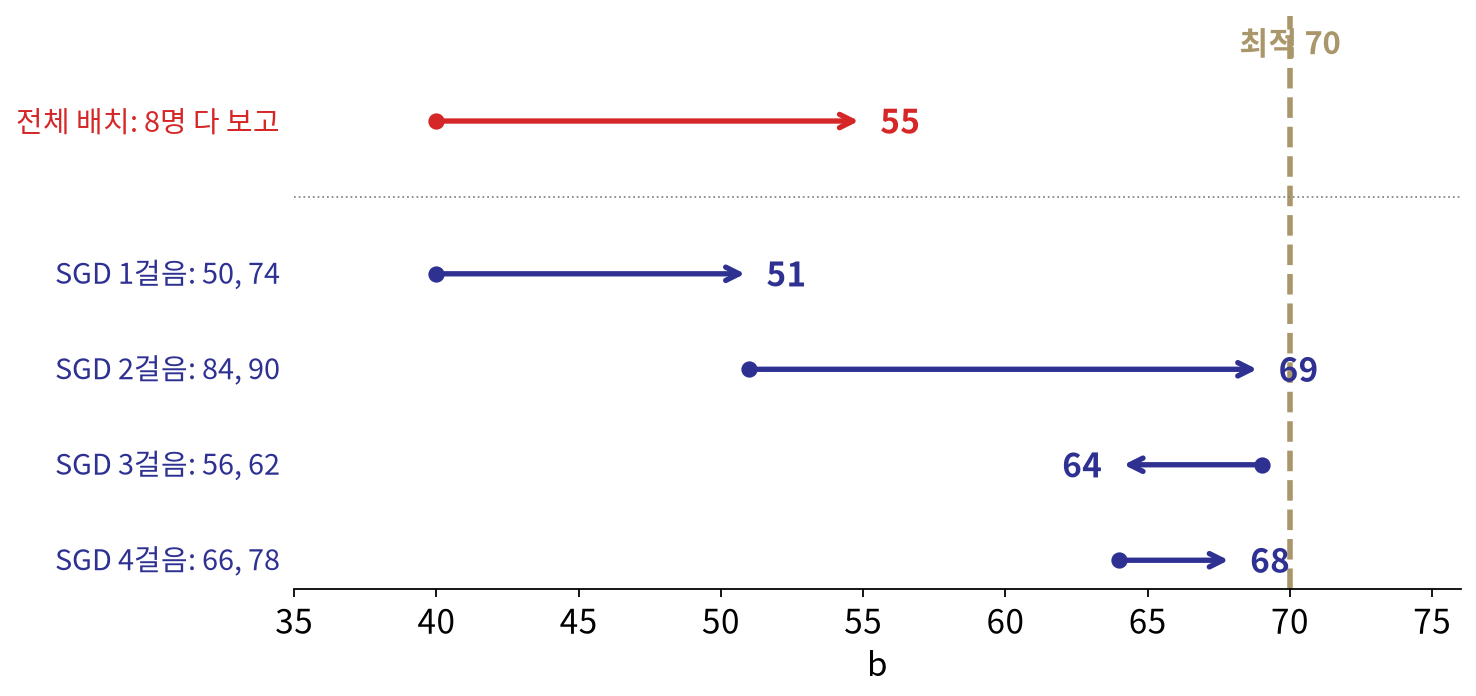
\includegraphics[width=0.78\linewidth]{sgd_epoch.png}\par\vskip0.2em
{\small 8명을 한 번씩 본 것은 같다. 전체 배치는 \kq{55}, SGD 는 4걸음 만에 \kb{68}}
\vfill
\note{8명의 점수로 1에폭을 직접 해 봅시다. 전체 배치는 8명을 다 보고 한 걸음, 40에서 55로 갑니다. SGD는 8명을 섞어 2명씩 4묶음으로 나눕니다. 첫 묶음 50점과 74점의 평균은 62, 기울기는 40 빼기 62, 마이너스 22이고, 0.5를 곱해 11만큼 올라가 51이 됩니다. 둘째 묶음 84점과 90점은 평균이 87이라 69까지 크게 올라갑니다. 셋째 묶음 56점과 62점은 평균이 59라서 오히려 64로 내려옵니다. 넷째 묶음 66점과 78점으로 68이 됩니다. 중간에 되돌아가는 걸음도 있지만, 같은 8명을 보고 55가 아니라 68, 최적값 70에 훨씬 가까워졌습니다.}
\end{frame}

% --- 2차원에서 보면
\begin{frame}{2차원에서 보면}
\vfill
\centering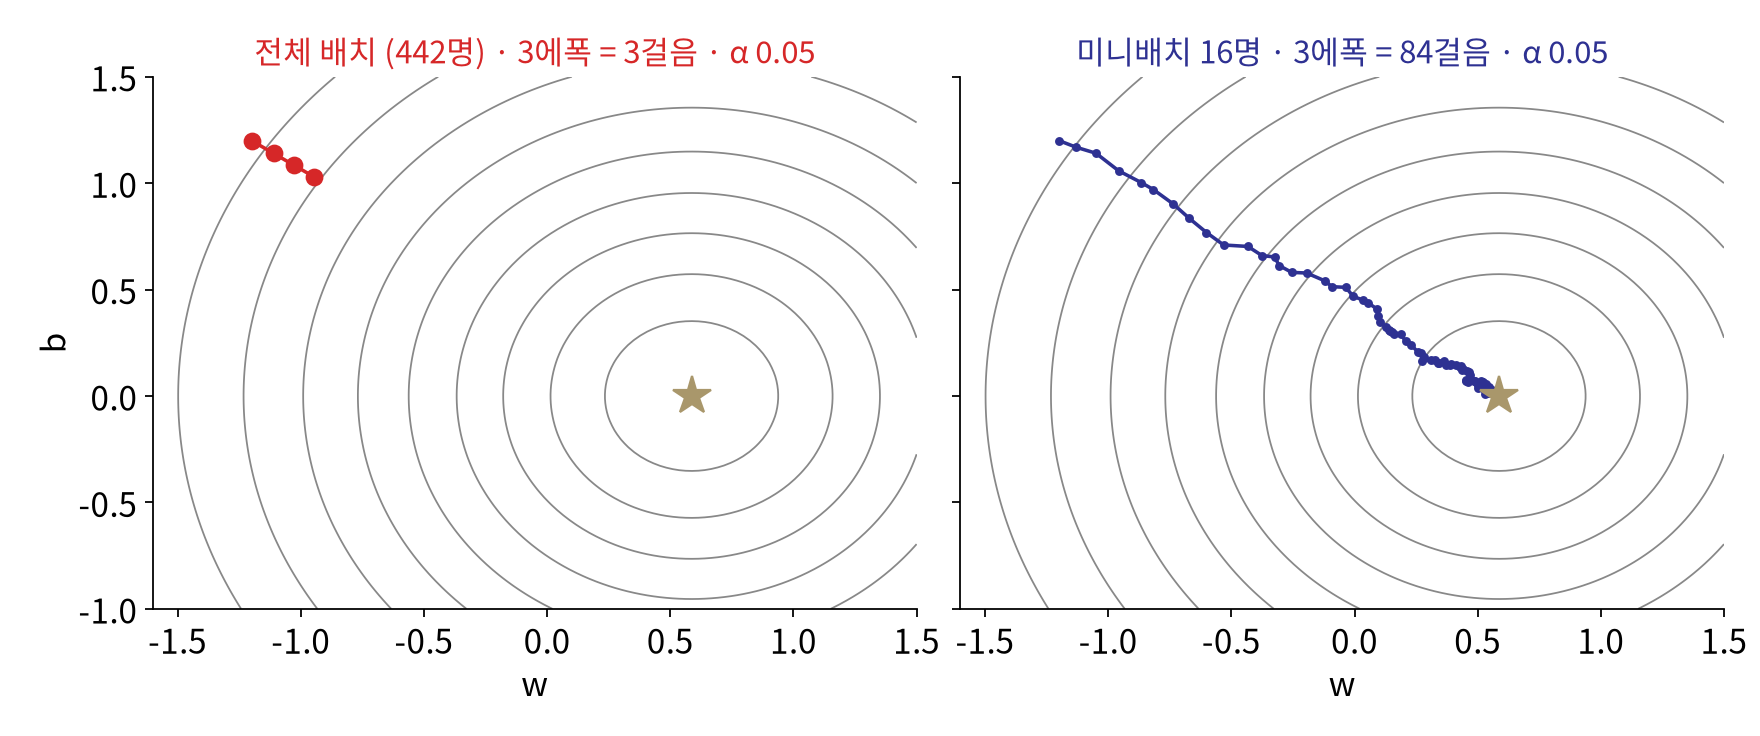
\includegraphics[width=0.8\linewidth]{sgd_paths.png}\par\vskip0.2em
{\small diabetes: BMI 로 1년 뒤 진행 정도 예측, $\hat y = wx+b$ \quad 같은 학습률 $\alpha=0.05$, 같은 3에폭 뒤 비용 $J$: 전체 배치 2.03, SGD \kb{0.33} (최솟값 0.33)}
\vfill
\note{1주차 선형회귀 실습의 diabetes 데이터로 w와 b 두 개를 학습시킨 경로입니다. 등고선은 비용 J이고 별이 최솟값입니다. 두 방법 모두 학습률 0.05로 같고, 데이터를 세 바퀴 봤습니다. 왼쪽 전체 배치는 3걸음뿐이라 출발점 근처에 있습니다. 오른쪽 SGD는 16명씩 84걸음을 걸어 별에 도착했습니다. 경로가 삐뚤빼뚤한 건 미니배치마다 기울기가 조금씩 틀리기 때문입니다. 3에폭 뒤 비용은 전체 배치 2.03, SGD 0.33으로 최솟값과 거의 같습니다. 이 문제는 아주 쉬운 2차 함수라서 전체 배치도 학습률을 크게 하면 빨리 갈 수 있습니다. 걸음 수 차이를 보여 주려고 학습률을 같게 맞춘 비교입니다.}
\end{frame}

\section{실전}
% --- 손글씨 6만 장 (MNIST)
\begin{frame}{손글씨 6만 장 (MNIST)}
\vfill
\centering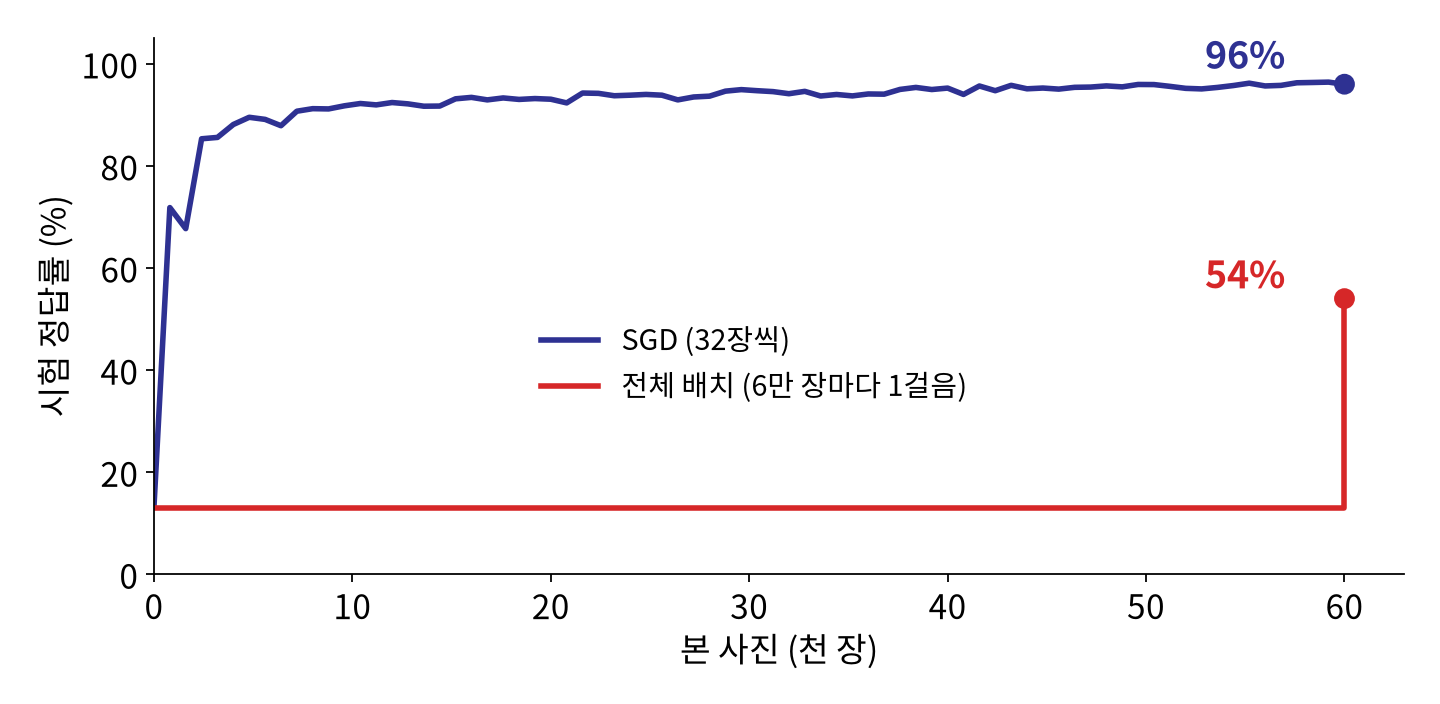
\includegraphics[width=0.66\linewidth]{sgd_mnist.png}\par\vskip0.2em
{\small SGD 는 800장(25걸음) 만에 72\% \quad 전체 배치로 96\% 에 닿으려면 \kq{318걸음 = 318에폭}}
\vfill
\note{처음 질문으로 돌아갑니다. 가로축은 지금까지 본 사진 수입니다. 전체 배치는 6만 장을 다 볼 때까지 제자리에 있다가, 마지막에 한 걸음 올라 54퍼센트가 됩니다. SGD는 32장마다 걸으니 처음부터 바로 올라갑니다. 800장, 25걸음 만에 이미 72퍼센트입니다. 전체 배치로 96퍼센트에 닿으려면 318걸음이 필요했는데, 걸음마다 6만 장을 보니 사진을 318바퀴 본 셈입니다. 두 방법 모두 학습률은 각자 가장 좋은 값으로 맞춘 공정한 비교입니다.}
\end{frame}

% --- 어림인데 왜 될까
\begin{frame}{어림인데 왜 될까}
\vfill
\centering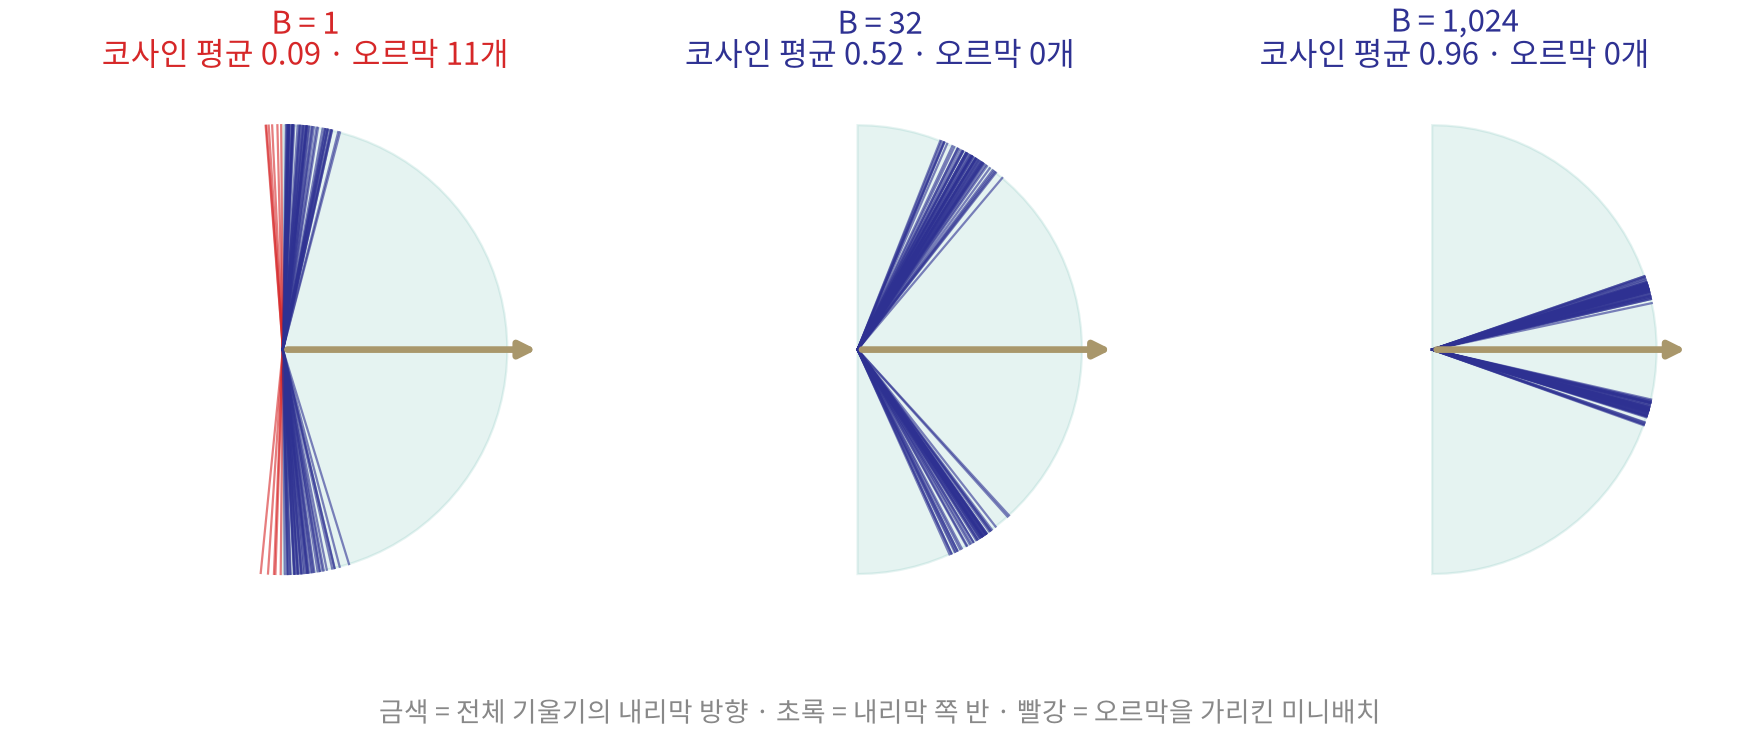
\includegraphics[width=0.84\linewidth]{sgd_fan.png}\par\vskip0.2em
{\small 학습 전 MNIST 신경망, 배치 크기마다 미니배치 100개의 기울기 방향을 전체 기울기와 비교 (코사인 유사도)}
\vfill
\note{MNIST 신경망에서 미니배치 기울기가 전체 기울기와 얼마나 같은 방향인지 재 봤습니다. 선 하나가 미니배치 하나이고, 금색 화살표가 전체 기울기로 본 내리막 방향입니다. 코사인 유사도가 0보다 크면 내리막 쪽 반, 초록 영역에 들어갑니다. 사진 1장이면 100개 중 11개가 오르막을 가리켰습니다. 32장이면 100개 모두 내리막 쪽이고, 1024장이면 거의 정확합니다. 32장 기울기는 꽤 틀리지만 늘 내리막 쪽이라서, 많이 걸으면 결국 내려갑니다.}
\end{frame}

% --- 배치 크기 고르기
\begin{frame}{배치 크기 고르기}
\vfill
\centering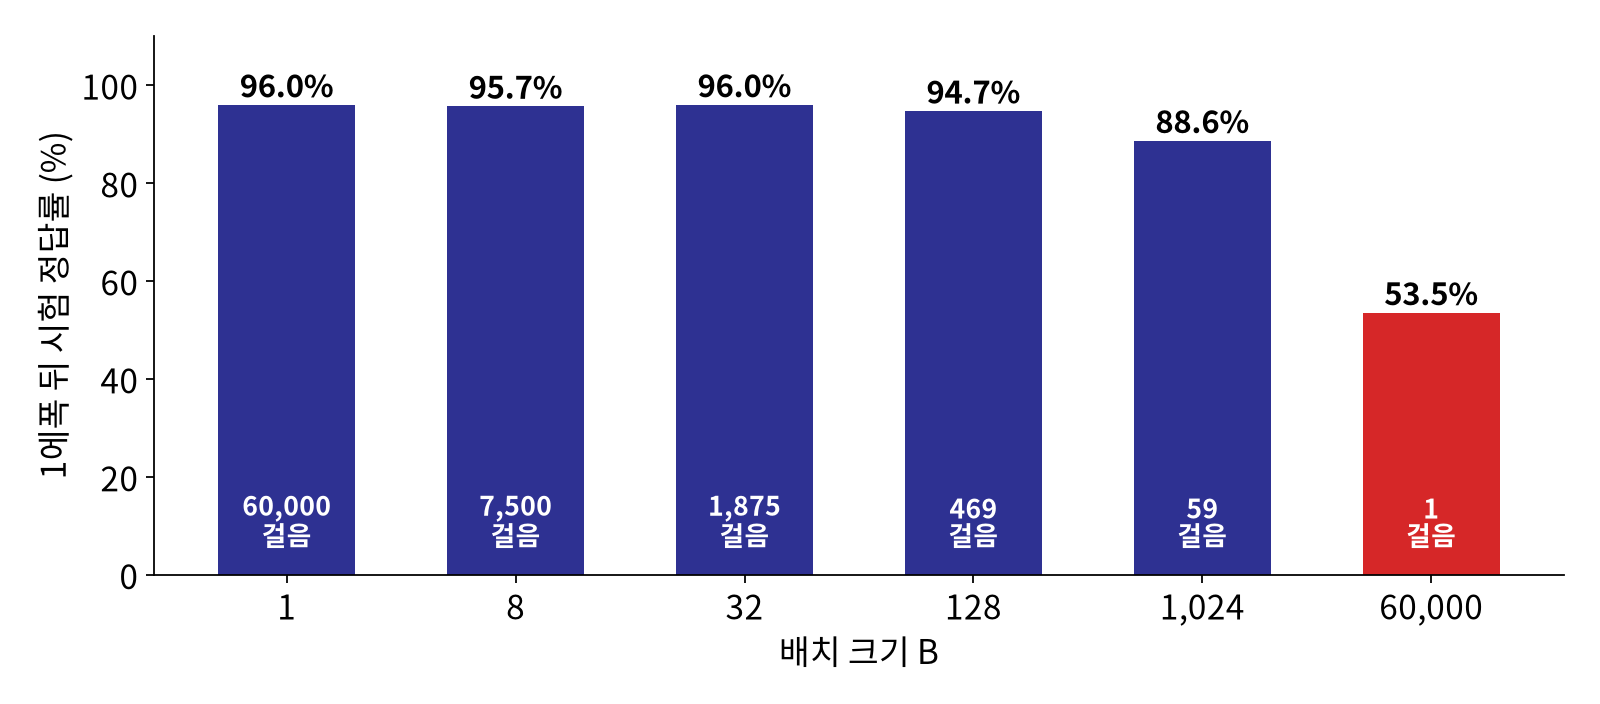
\includegraphics[width=0.66\linewidth]{sgd_batch.png}\par\vskip0.2em
{\small 1에폭 시간 (이 실험의 CPU): $B=1$ 4.5초, $B=32$ 0.3초 \quad 같은 6만 장인데 한 장씩은 \kq{15배} 느리다}\\[0.2em]
{\footnotesize 작은 $B$: 걸음 많음 · 많이 흔들림 \qquad 큰 $B$: 정확함 · 걸음 적음 · 한 번에 여러 장을 동시에 계산}
\vfill
\note{배치 크기를 1부터 전체 6만까지 바꿔 1에폭씩 학습시켰습니다. 1, 8, 32는 모두 96퍼센트 안팎이고, 128부터 떨어지기 시작해 전체 배치는 54퍼센트입니다. 그럼 1장씩이 가장 좋을까요? 시간을 재 보면 1장씩은 4.5초, 32장씩은 0.3초입니다. 같은 6만 장인데 15배 느립니다. 컴퓨터는 여러 장을 한 번에 묶어 계산하는 게 훨씬 빠르기 때문입니다. 그래서 실전에서는 정확도와 속도 사이에서 수십에서 수백 장 정도의 배치를 고릅니다. GPU를 쓰면 이 차이가 더 커집니다.}
\end{frame}

% --- 1951년부터
\begin{frame}{1951년부터}
\vfill
\centering
{\Large Robbins · Monro (1951)}\\[0.4em]
{\normalsize Robbins \& Monro, \emph{A Stochastic Approximation Method}, Annals of Mathematical Statistics}\\[1.2em]
틀린 값으로 여러 번 고쳐도 \kb{평균적으로 맞으면} 답에 다가간다\\[1.2em]
{\small 지금의 딥러닝 학습은 거의 모두 미니배치 위에서 걷는다 $\rightarrow$ 이번 주: 모멘텀 · Adam}
\vfill
\note{이 생각은 1951년 통계학자 Robbins와 Monro의 확률적 근사 논문에서 시작됐습니다. 매번 잡음이 섞인 값으로 고쳐도, 그 값이 평균적으로 맞고 걸음 크기를 알맞게 줄여 가면 답에 다가간다는 내용입니다. 오늘 본 미니배치 기울기의 기댓값 식이 바로 그 조건입니다. 지금의 딥러닝 학습은 거의 모두 미니배치 기울기 위에서 걷습니다. 이번 주에 배울 모멘텀과 Adam도 SGD의 걸음 방법을 고친 것입니다.}
\end{frame}

\section{연습}
% --- 문제풀이
\begin{frame}{문제풀이}
\vfill
\begin{enumerate}
\item 데이터 50,000개, 배치 크기 100. 1에폭은 몇 걸음인가? 10에폭은?\vskip0.8em
\item 점수 60, 64, 80, 84 인 4명, 모델 $\hat y=b$, 지금 $b=50$.\\ (a) 전체 기울기는? \; (b) 미니배치 \{60, 64\} 의 기울기는? \; (c) $\alpha=0.5$ 로 (b) 한 걸음 가면 $b$ 는?\vskip0.8em
\item 4명에서 2명을 고르는 6가지 쌍의 기울기를 모두 구해 평균이 (a) 와 같은지 확인하라.
\end{enumerate}
\vfill
\note{문제 세 개를 풀어 봅시다. 1번 답. 5만 나누기 100, 500걸음이고, 10에폭은 5,000걸음입니다. 2번 답. 평균 점수가 72이므로 전체 기울기는 50 빼기 72, 마이너스 22입니다. 미니배치 60과 64의 평균은 62이니 기울기는 마이너스 12입니다. 한 걸음 가면 50 빼기 0.5 곱하기 마이너스 12, 56이 됩니다. 3번 답. 여섯 쌍의 평균 점수는 62, 70, 72, 72, 74, 82이고, 기울기는 마이너스 12, 20, 22, 22, 24, 32입니다. 더하면 마이너스 132, 6으로 나누면 마이너스 22로 전체 기울기와 같습니다.}
\end{frame}

% --- 실습
\begin{frame}{실습}
\vfill
\centering\begin{tabular}{rl}\large 1 & 미니배치 기울기 1,000개를 뽑아 평균이 전체 기울기와 같은지 확인 · 배치 크기별 흩어짐\\[0.5em]\large 2 & SGD 직접 구현 (섞기 · 자르기 · 걷기) 후 전체 배치와 비용 비교\\[0.5em]\large 3 & PyTorch 로 MNIST 54\% vs 96\% 재현 · 배치 크기 바꿔 보기\end{tabular}\vskip1em diabetes (442명, scikit-learn 내장) · MNIST 손글씨 (6만 장)\\[0.4em]\href{https://colab.research.google.com/github/SuminHan/book-ml/blob/main/slides/v2/ml1/week02/sgd/lab/sgd.ipynb}{\textcolor{ksagolddk}{▶ Colab에서 실습 노트북 열기}}
\vfill
\note{실습은 세 부분입니다. 첫째, diabetes 데이터에서 미니배치 기울기를 천 개 뽑아 평균이 전체 기울기와 같은지, 배치 크기에 따라 얼마나 흩어지는지 확인합니다. 둘째, SGD를 직접 구현합니다. 섞기, 자르기, 걷기 세 줄을 채우면 됩니다. 셋째, PyTorch로 오늘 처음 본 MNIST 실험을 그대로 재현하고 배치 크기를 바꿔 봅니다.}
\end{frame}

\section{정리}
% --- 정리
\begin{frame}{정리}
\vfill
\centering\large\begin{tabular}{l}전체 기울기 \quad 데이터 하나하나의 기울기의 평균\\[0.5em]미니배치 기울기 \quad $B$ 개만 뽑아 어림, \kb{평균적으로 정확} ($\mathbb E[g_{\mathcal B}]=\partial J/\partial w$)\\[0.5em]SGD \quad 에폭마다 섞고, $B$ 개씩 잘라 걷는다 (1에폭 $= m/B$ 걸음)\\[0.5em]배치 크기 \quad 작으면 흔들림 · 크면 걸음 수 부족, 속도까지 보고 고른다\end{tabular}
\vfill
\note{정리합니다. 전체 기울기는 데이터 하나하나의 기울기의 평균입니다. 미니배치 기울기는 그중 B개만 뽑아 어림한 것이고, 기댓값이 전체 기울기와 같아서 평균적으로 정확합니다. SGD는 에폭마다 데이터를 섞고 B개씩 잘라 걷습니다. 배치 크기가 작으면 많이 흔들리고, 크면 같은 데이터로 걸을 수 있는 걸음 수가 줄어듭니다. 계산 속도까지 함께 보고 고릅니다.}
\end{frame}
\end{document}
